\subsection{\secState{R}Constrained Trajectory Expansion}\label{s:constrainedTrajectoryExpansion}

\paragraph{Motivation:} \emph{Purpose} of \emph{Navigation} is to move forward to \emph{Goal Waypoint} in \emph{Mission}. \emph{Structure} of \emph{Avoidance Grid} is designed to enable \emph{forward} and \emph{turning} maneuvers. The \emph{Avoidance Grid} is organized in \emph{Layers} characteristic by same distance from \emph{Avoidance Grid Origin}. 

Survey of motion planning algorithm was given in \cite{goerzen2009survey}. The ideal candidate for propagation algorithm is \emph{Wave-front} algorithm propagating \emph{Trajectory tree} through Layers. Due the \emph{Avoidance Grid} onion like layers, there is possibility to implement turn maneuver through layers iterative and effectively .

\begin{figure}[H]
    \centering
    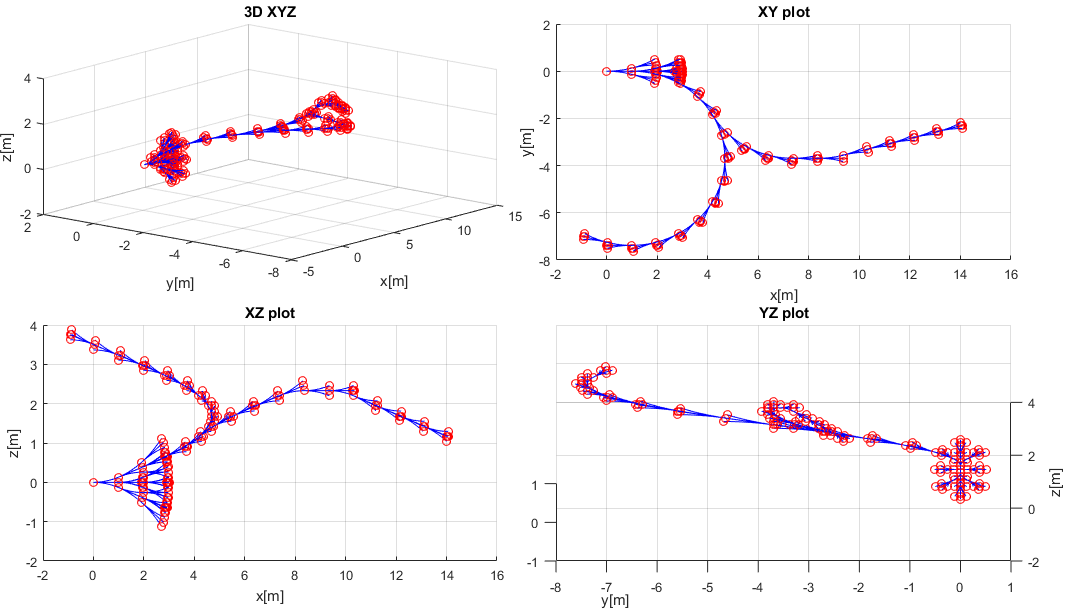
\includegraphics[width=0.9\linewidth]{\FIGDIR/RS001RapidExplorationTreeExampleShrink} 
    \caption{\emph{Rapid Exploration tree as result of \emph{Constrained trajectory expansion}}.}
    \label{fig:rapidExplorationTrajectoryTree}
\end{figure}

\paragraph{Rapid Exploration Tree} (fig. \ref{fig:rapidExplorationTrajectoryTree}) was selected, because it enables \emph{Movement Automaton Utilization} and \emph{Property Binding}. Similar approach was used for space exploration \cite{plaisant2002spacetree}. 

\paragraph{The example} (fig. \ref{fig:rapidExplorationTrajectoryTree}) shows a \emph{Rapid Exploration Tree} in \emph{Free Space} containing \emph{Waypoint Navigation Path} and \emph{Turn Away Path}. Both paths are starting in same \emph{Root Node} (red circle) which was expanded with simple \emph{Movement Automaton} (bunch of nodes originating from one node are showing way of expansion). The connection (blue line) between two nodes (red circles) represents \emph{Trajectory portion} for \emph{Executed Movement}.

\paragraph{Rapid Exploration Tree Node} will contain following information:
\begin{enumerate}
    \item \emph{Initial state} - root entry point, used in state evolution calculation.
    \item \emph{Trajectory (state evolution)} - trajectory passing through \emph{state space} in local coordinate frame of \emph{Avoidance Grid}.
    \item \emph{Buffer} (applied movements) - ordered list of \emph{executed movements} applied on \emph{initial state} to obtain \emph{state evolution}.
    \item \emph{Cost} - calculated for \emph{state evolution} based on \emph{predefined cost function}. 
    \item \emph{Footprint} - ordered set of \emph{passing cells} in \emph{Avoidance Grid}.
    \item \emph{Parent Node Reference} - tree reference for parent node, not in case of \emph{root node}.
    \item \emph{Other Bounded Properties} - value list of other properties, depending on \emph{Expansion Constraints} and \emph{Reachability} evaluation algorithm.
\end{enumerate}

\paragraph{Wave-front propagation of Rapid Exploration Tree} is given in (alg. \ref{alg:Wavefront Propagation}). 

The \emph{Avoidance Grid} have UAS with \emph{position $\in$ Initial State} at the \emph{origin}. The \emph{Grid Layer} is a column ordered set of cells with same \emph{Mean distance} from origin. \emph{Grid Layers} are indexed from origin starting with $1$, there is maximum of \emph{i $\ge$ 1} layers.

\paragraph{Step: Initialization} contains base structure preparation like follows:
\begin{enumerate}
    \item \emph{Avoidance Grid} - Space containing \emph{Reach set} (def. \ref{def:ContainedReducedReachSet}).
    \item \emph{Movement Automaton} - Used as \emph{Predictor}, consuming \emph{buffer} containing \emph{Movements} to generate $Trajectory(initialState,buffer)$.
    
    \item \emph{Reach Set} -  tree consisting from \emph{Wave-frontNodes} representing the end point of $Trajectory(initialState,buffer)$ where each \emph{Edge} represents \emph{one Movement application}. The root is set as node containing \emph{Initial State}.
\end{enumerate}

\noindent Function \emph{initializeReachSet(root,stack,grid,automaton)} will take the root and enforces \emph{full wavefornt propagation} to \emph{First Layer}.


\paragraph{Step: Wave-front Propagation} is forced propagation of trajectories from layer $i$ to layer $i+1$. The process goes as follows:
\begin{enumerate}
    \item \emph{Selection of Feasible candidates} - function \emph{[candidates,leftovers] = ExpansionConstraints.select(stack)} for working layer, row and cell selects \emph{feasible trajectory nodes} ordered by \emph{Cost function}. The \emph{Example of Cost Function} can be \emph{Trajectory Smoothness} (def. \ref{def:SmoothnessRatingForTrajectory}).
    
    \item \emph{Expansion of Candidates} - for each \emph{candidate} function \emph{candidate.expandNode (automaton)} is invoked. This function will expand \emph{Candidate Node structure} by appending \emph{Full Trajectory Tree Evolution} until each \emph{Leaf Trajectory} reaches \emph{Next Layer}. Simply put \emph{Par rent Node} \emph{Node(initialState, buffer, cost, footprint )} buffer is appended by movements until the next layer is reached.
    
    \item \emph{Leftovers purge} - function \emph{reachSet.purge(leftovers)} removes unexpanded \emph{Nodes} leading to cell, effectively  removing trajectories which does not  lead to \emph{next layer}.
    
    \item \emph{Append Reach Set} - function \emph{reachSet.append(leafs)} puts newly created \emph{Nodes (Trees)} into \emph{Reach Set} structure. The \emph{Wave-front Propagation} for one cell is finished.
\end{enumerate}

\paragraph{Step: After Layer Propagation Purge} is covered by function \emph{reachSet.purgeSame- Footprint()} which takes trajectories with same footprint and keeps some of them based on \emph{Selection criteria}, more in (sec. \ref{s:chaoticReachSet}, \ref{s:harmonicReachSet}). \emph{Pruning methods} over \emph{Large Decision Trees} are \emph{fast} and \emph{viable} \cite{mingers1989empirical}.

\begin{note}
    \emph{Reach Set} is usually computed \emph{Prior the Flight} for \emph{some Initial State} in \emph{Local Coordinate Frame} in \emph{right had coordinate frame} with $X^+$ used as \emph{main axis}.
\end{note}


\begin{algorithm}[H]
    \SetKwInOut{Input}{Input}\SetKwInOut{Output}{Output}
    \Input{Node(initialState,buffer=$\varnothing$,cost=0,footprint=$\varnothing$),
           AvoidanceGrid, ExpansionConstraints, MovementAutomaton(movementSet)
    }
    \Output{ReachSet(AvoidanceGrid)}
    \BlankLine
    \# Initialization Sequence\;
    grid=AvoidanceGrid, automaton=MovementAutomaton, root = Node\;
    reachSet = initializeReachSet(root,stack,grid,automaton)\;
    \BlankLine
    \# Main Expansion through, layers (i), rows (j), cells(k)\;
    \For{layer($1\dots i$) \emph{in} grid}{
        \For{row($1\dots j$ \emph{in} layer)}{
            \For{cell($1 \dots k$) \emph{in} row}{
                \BlankLine
                \# apply selection criteria \;
                [candidates,leftovers] = ExpansionConstraints.select(stack)\;
                \BlankLine
                \# collect expansions \;
                leafs = []\;
                \For{candidate \emph{in} Candidates}{
                    leafs= [leafs, candidate.expandNode(automaton)];
                }
                reachSet.purge(leftovers)\;
                reachSet.append(leafs)\;
            }
        }
        reachSet.purgeSameFootprint()\;
    }
    \caption{\emph{Wave-front propagation} of \emph{Rapid Exploration Tree} to form \emph{Reach Set}.}
    \label{alg:Wavefront Propagation}
\end{algorithm}





